\section{Introduction}
\label{sec:intro}

%% Teaser figure (one column).
%% Layout follows the teaser of the Image Analogies paper:
%%   top row    -- A : A'   (reference normal render  :  reference tactile normal video)
%%   bottom row -- B : B'   (query normal render      :  predicted tactile normal video)
%% Replace the \rule placeholder below with the actual graphic.
\begin{figure}[t]
  \centering
  % 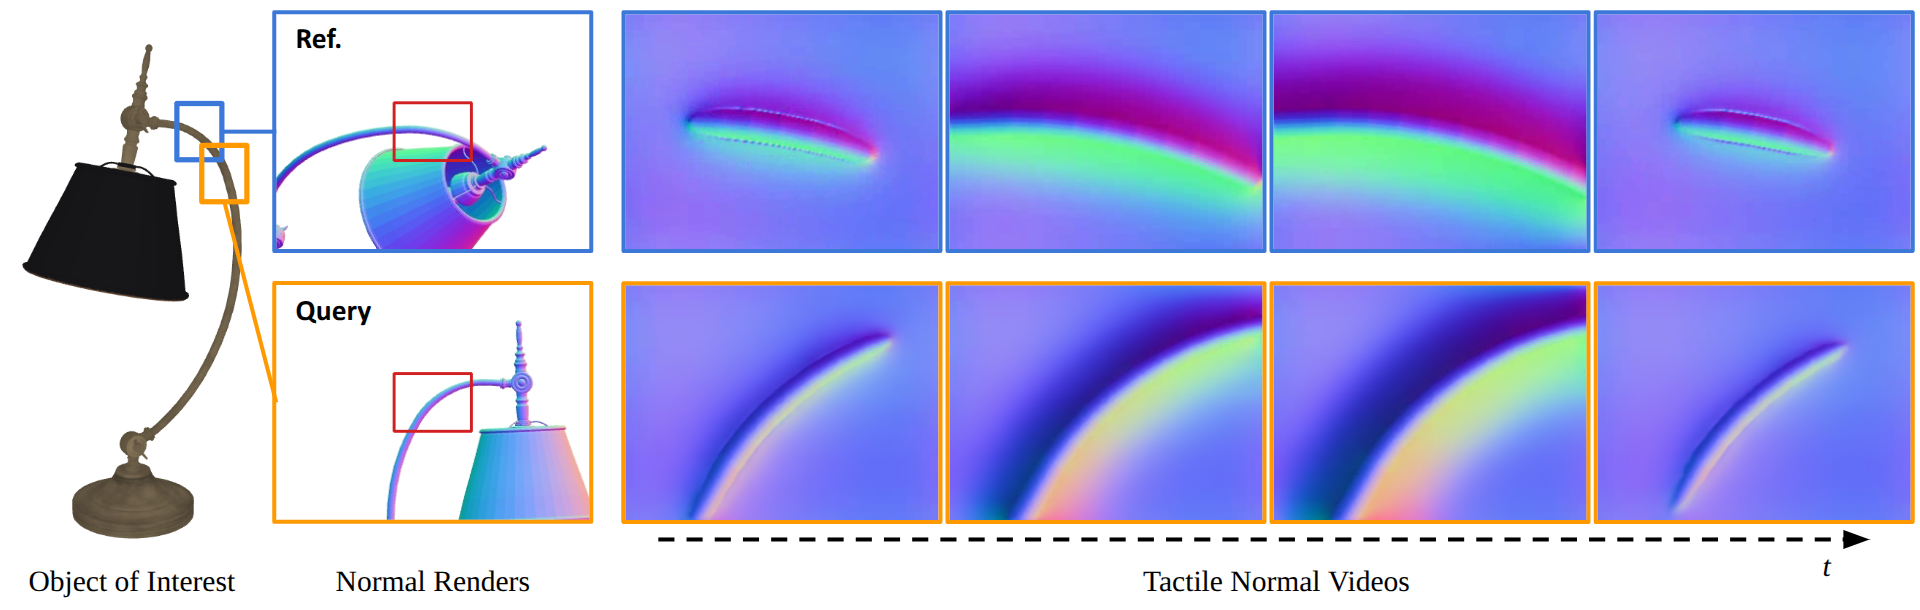
\includegraphics[width=\linewidth]{figures/teaser.pdf}
  \rule{\linewidth}{4.2cm}% PLACEHOLDER -- remove when the real figure is dropped in
  \caption{\textbf{Tactile analogies.} Given a reference touch recorded on an object (top right)
    together with the surface geometry at the location it was taken from (top left), we predict
    the tactile signal that the sensor would measure at a new, previously untouched location
    (bottom right) given only the geometry there (bottom left). We represent a touch as a
    \emph{tactile normal video}, which records how the sensor's deformable gel bends over the
    course of a press, so the prediction is a short video rather than a single frame. The
    relationship between the two columns is the analogy our method must transfer: as the reference
    geometry is to the reference touch, so the query geometry is to the touch we synthesise.}
  \label{fig:teaser}
\end{figure}


Humans have a remarkable ability to imagine what it would feel like to touch an object at a
particular location. Looking at a ceramic mug, we already know that its glazed side will feel
smooth and that the unglazed ring at its base will feel rough and gritty, long before our fingers
arrive there. This ability lets one to plan a grasp, avoid an obstacle, and build a holistic picture of the
fine-grained surface detail of a scene without having to physically touch every location.
One important aspect to note here is that the touch one imagines is \textit{not} a single snapshot in time.
Rather, it is a mental simulation on the continous dynamics of how our non-rigid skin would progressively deform during contact.

Why is this possible at all for humans? 
One key reason is due to the fact that tactile information is highly repetitive and predictable. 
Object surfaces are often made of a small number of materials and recurring geometric motifs,
so a handful of touches already reveals most of what the rest of an object will feel like. 
What remains is to work out \emph{which} previously felt sensation applies at a new
location, and \emph{how} it should be transformed to account for the change in surface geometry.

In this paper we aim to teach machines the same capacity. We introduce the task of finding
\emph{tactile analogies}: given a set of reference touches captured on an object during contact,
the goal of tacile analogies is to predict the tactile signal at new, untouched locations (Fig.~\ref{fig:teaser}).
We represent a touch as a \emph{tactile normal video}, a sequence of frames that encodes the surface normals of
the visuo-tactile sensor's deformable gel over the duration of a press. 
Tactile normal videos are easy to obtain in practice, because the mapping from the raw color measurements of a modern visuo-tactile 
sensor to gel normals is by design nearly one-to-one. Sensor manufacturers such as
GelSight~\cite{gelsight} ship colour-to-normal conversion as part of their SDK. To
predict gel normals at a new location, we render surface normal maps at both the reference and
query sensor poses over multiple scales, and compare these renderings to recover a
mapping that transfers reference tactile videos to the query location.

Our task therefore resonates with the \emph{analogy-based synthesis} idea of the seminal Image
Analogies paper~\cite{imageanalogies}: observe a transformation on one pair of images, then predict how the transformation would unfold in a new input. 
For our setting, the observed side is the normal map rendered at each sensor pose, and the target to synthesize 
is a \emph{high-dimensional tactile video} rather than a still image. 
Put differently, we ask for an analogy between surface geometry and the temporal signal (i.e., touch) that arises through interaction with that geometry.

There exist several factors that make our task challenging.
First of all, the physics of contact is complicated, since the gel deforms
non-rigidly and its response depends on material properties that are not observable from geometry
alone.
Secondly, the search space is large: one must decide which of the available reference touches is relevant 
\emph{and} how that reference should be mapped onto the query sensor pose.
Finally, there is no large-scale dataset of paired touches at controlled locations on which a model could simply be
trained end-to-end.

To address these problems, our solution takes a modular approach, where retrieval and coarse prediction reduces the large search space 
and the learning-based refinement focuses on enhancing video predictions to accurately model gel dynamics.
As the first step, our method compares 2D foundation model features~\cite{dinov3} between the reference 
normal renders and the query to obtain a single promising reference location.
Then for coarse alignment, we use pre-trained local feature matchers on the
normal map renderings, which show highly accurate match success rates despite being out of
distribution with respect to the multi-view RGB imagery the matchers are trained on. The local
feature matches are used to find a homography that aligns the two normal maps, reference and
query, which is further used to warp the tactile videos to produce an initial transfer. For
refinement, we propose training a refinement network that takes initially warped tactile normal
videos and is trained to regress the ground-truth query tactile video. The network is responsible
for learning the subtle gel deformation dynamics and for correcting the misalignments from the
initial transfer.

Our experiments show that our pipeline outperforms all the tested baselines, while exhibiting a
small runtime. We further demonstrate applications in 3D reconstruction and visuo-tactile sensor
simulation, which could be used for fine-grained surface understanding and could help embodied
agents that are pre-trained on visuo-tactile sensor inputs.

\vspace{0.5em}
\noindent Our contributions are:
\begin{itemize}
  \setlength{\itemsep}{0pt}
  \item We introduce the task of tactile analogies, namely, predicting tactile videos at
        untouched locations from a set of reference touches, together with a benchmark to evaluate it
        built on ObjectFolder.
  \item We propose a simple and efficient coarse-to-fine solution that combines geometry-based
        retrieval, feature-matching alignment, and a lightweight refinement network.
  \item We show that our method outperforms baselines adapted from prior tactile prediction work.
  \item We demonstrate applications in 3D surface reconstruction and in simulating visuo-tactile
        sensor measurements without physical contact.
\end{itemize}
